\subsection{EEG Recording and Analysis}
To compute distinctive feature weights used in estimating the misperception
transducer as shown in Eqs.~\ref{eq:dfdist} and~\ref{eq:eegdist},
recordings of cortical activity in response to non-native phones were
made using EEG. Signals were acquired using a BrainVision actiCHamp 
system with 64 channels and 1000 Hz sampling rate.
All methods were approved by the University of Washington Institutional
Review Board.

Auditory stimuli used to evoke the electrocortical responses comprised
consonant-vowel (CV) syllables representing three languages: English,
Dutch and Hindi. The inclusion of only two non-English languages in the
auditory stimuli was dictated by the relatively high number of
repetitions required to achieve good signal-to-noise ratio from averaged
EEG recordings. The choice of Dutch and Hindi was governed by their
inclusion in the SBS subset used to train the misperception G2P as
described in Section~\ref{sec:MC}, and the relative similarities
between their phoneme inventories and the phoneme inventory of English.
In particular, we chose languages with relatively many (Hindi) or few
(Dutch) ``many-to-one mappings'' between the non-English phoneme
inventory and the phoneme inventory of English, estimated based on 
distinctive feature representations of the phonemes in each language 
(as given in the PHOIBLE database~\cite{PHOIBLE}). Such 
``many-to-one mappings'' are expected to pose a problem for the 
non-native transcription task being modeled by the misperception 
transducer, so to test the limits of our design we chose languages that 
differed greatly in this property. 
%% rest of this paragraph could probably be cut if necessary
Note that, although Hindi podcasts were not included in the SBS training
data described in Section~\ref{sec:data}, colloquial spoken Hindi and
Urdu are extremely similar phonologically~\cite{Kachru90}, and
considering that the auditory stimuli for the EEG portion of this
experiment are simple CV syllables, it is reasonable to consider Hindi
and Urdu as equivalent for the purpose of computing feature weights for
the misperception transducer.

%% This next section, including tab:m2o, seems like more detail than
%% is necessary; the explanation above as to **why** we chose Hindi and
%% Dutch (combined with tab:eegphones) seems sufficient here, without
%% going into the extra details of **how** we settled on those two.
Language similarity was defined as the number of many-to-one mappings
($N_{M2O}(\mathbb{\Phi})$) between the English phoneme inventory
($\mathbb{\Psi}$) and the non-native phoneme inventory $\mathbb{\Phi}$.
Using distinctive feature representations of the phonemes in each
inventory (as given in the PHOIBLE database \cite{PHOIBLE}), a
many-to-one mapping was defined by finding, for each
non-native phoneme $\phi$, the English phoneme $\psi^*(\phi)$ to which
it is most similar:
\begin{equation}
  \psi^*(\phi) = \argmin \sum_k \delta\left(f_k(\psi)\ne f_k(\phi)\right)
\end{equation}
The number of many-to-one collisions is then defined as
\begin{equation}
  N_{M2O}(\mathbb{\Phi})=\frac{1}{|\mathbb{\Psi}|}\sum_{\phi_1\ne\phi_2}
  \delta\left(\psi^*(\phi_1)=\psi^*(\phi_2)\right)
\label{eq:m2o}
\end{equation}
where $|\mathbb{\Psi}|$ is the size of the English phoneme inventory.
The frequency of many-to-one mappings is listed in
Table~\ref{tab:m2o} for several languages.

\begin{table}
  \centerline{\begin{tabular}{|lr|lr|lr|}\hline
    $\mathbb{\Phi}$ & $N_{M2O}(\mathbb{\Phi})$ &
    $\mathbb{\Phi}$ & $N_{M2O}(\mathbb{\Phi})$ &
    $\mathbb{\Phi}$ & $N_{M2O}(\mathbb{\Phi})$ \\ \hline
    spa & 0.862 & yue & 1.280 & cmn & 1.531 \\
    por & 1.152 & jpn & 1.333 & amh & 1.844 \\
    nld & 1.182 & vie & 1.393 & hun & 1.857 \\
    deu & 1.258 & kor & 1.429 & hin & 2.848 \\\hline
  \end{tabular}}
  \caption{Frequency of many-to-one mappings $N_{M2O}(\mathbb{\Phi})$
    between phoneme inventory $\mathbb{\Phi}$ and the inventory of
    English. Languages are represented by their ISO 639-3 codes.}
  \label{tab:m2o}
\end{table}

To construct the auditory stimuli, two vowels and several consonants
were selected from the phoneme inventory of each language (18 consonants
for English, 17 for Dutch, and 19 for Hindi). Choice of consonants was
made so as to emphasize differences in the many-to-one relationships
between English-Dutch and English-Hindi, while maintaining roughly equal 
numbers of consonants for each language. The consonants chosen for each 
language are given in Table~\ref{tab:eegphones}; the vowels chosen were 
the same for all three languages (/a/ and /e/).

\begin{table}
  \centering
  \setlength{\tabcolsep}{0.3em}
  \setlength\extrarowheight{2pt}
  \begin{tabular}{|l||cc|cccc|cc|c|cccc|cc|c|c|c|c|c|c|c|c|c|cc|c|c|c|}\hline
    Language & \multicolumn{29}{c|}{Consonant phones used in the EEG experiment}\\ \hline
    eng & \multicolumn{2}{c|}{p} & \multicolumn{4}{c|}{t} & \multicolumn{2}{c|}{k} & \textipa{p\super h} & \multicolumn{4}{c|}{\textipa{t\super h}} & \multicolumn{2}{c|}{\textipa{k\super h}} & \textipa{tS} & \textipa{tS\super h} & f & \textipa{T} & \textipa{S} & v & \textipa{D} & z & m & \multicolumn{2}{c|}{n} & l & \textipa{\*r} & \\ \hline
    nld &  \multicolumn{2}{c|}{p} & \multicolumn{4}{c|}{t} & \multicolumn{2}{c|}{\textipa{G}} & \textipa{p\super h} & \multicolumn{4}{c|}{\textipa{t\super h}} & \multicolumn{2}{c|}{\textipa{k\super h}} & & \textipa{tS\super h} & f & & \textipa{S} & v & & z & m & \multicolumn{2}{c|}{n} & l & \textipa{\;R} & j \\ \hline
    hin &  p & b & \textipa{\|[t} & \textipa{\|[d} & \textipa{\:t} & \textipa{\:d} & k & \textipa{g} & \textipa{b\super H} & \textipa{\|[t\super h} & \textipa{\:t\super h} & \textipa{\|[d\super H} & \textipa{\:d\super H} & \textipa{k\super h} & \textipa{g\super H} & & & & & & \textipa{V} & & & m & \textipa{\|[n} & \textipa{\:n} & & & \\ \hline
  \end{tabular}
  \caption{Consonant phones used in the EEG experiment represented using
  IPA. Vertical alignment of cells suggests many-to-one mappings
  expected based on distinctive feature values from PHOIBLE.}
  \label{tab:eegphones}
\end{table}

Two native speakers of each language (one male and one female) were
recorded (44100 sample rate, 16 bit depth) speaking multiple repetitions of the set of CV syllables for
their language. Three tokens of each unique syllable were excised from
the raw recordings (24414 downsampled, RMS normalized)
Recorded syllables had an average duration of 400~ms, and were presented
via headphones to one monolingual American English listener.
The stimuli were presented in 9 blocks of 15 minutes per block, for a
total of 135 minutes.  Syllables were presented in random order with an
inter-stimulus interval of 350~ms. 21 repetitions of each syllable
were presented, for a grand total of 9072 syllable presentations.

%% TODO: get number of ms where epoch started (MM to email GDL)
EEG recordings were divided into 500 ms epochs beginning XXX ms before
each syllable onset.
The epoched data were coded with a subset of distinctive features
that minimally defined the phoneme contrasts of the English consonants.
Where more than one choice of features was sufficient to define those
contrasts, preference was given to features that reflect differences
in temporal as opposed to spectral features of the consonants, due to
the high fidelity of EEG at reflecting temporal envelope properties of 
speech.~\cite{Liberto15} The final set of features chosen was:
continuant, sonorant, delayed release, voicing, aspiration, labial,
coronal, and dorsal.
% In other words, differences in the temporal amplitude envelope of
% consonants have a better chance of being recoverable after being
% filtered through a human auditory system and cortex than do differences
% that are purely spectral in nature; to the extent that spectral
% information in speech is preserved in an EEG signal, it will have been
% transformed to be spatially coded across populations of neurons.

Epoched and feature-coded EEG data {\em for the English syllables only}
were used to train a support vector machine classifier for each feature.
The classifiers were then used (without re-training) to classify the
EEG responses to the Dutch and Hindi syllables.
Fig.~\ref{fig:eeg_svm_eers} shows equal error rates of these
classifiers when applied to the three languages.

\begin{figure}
  \centerline{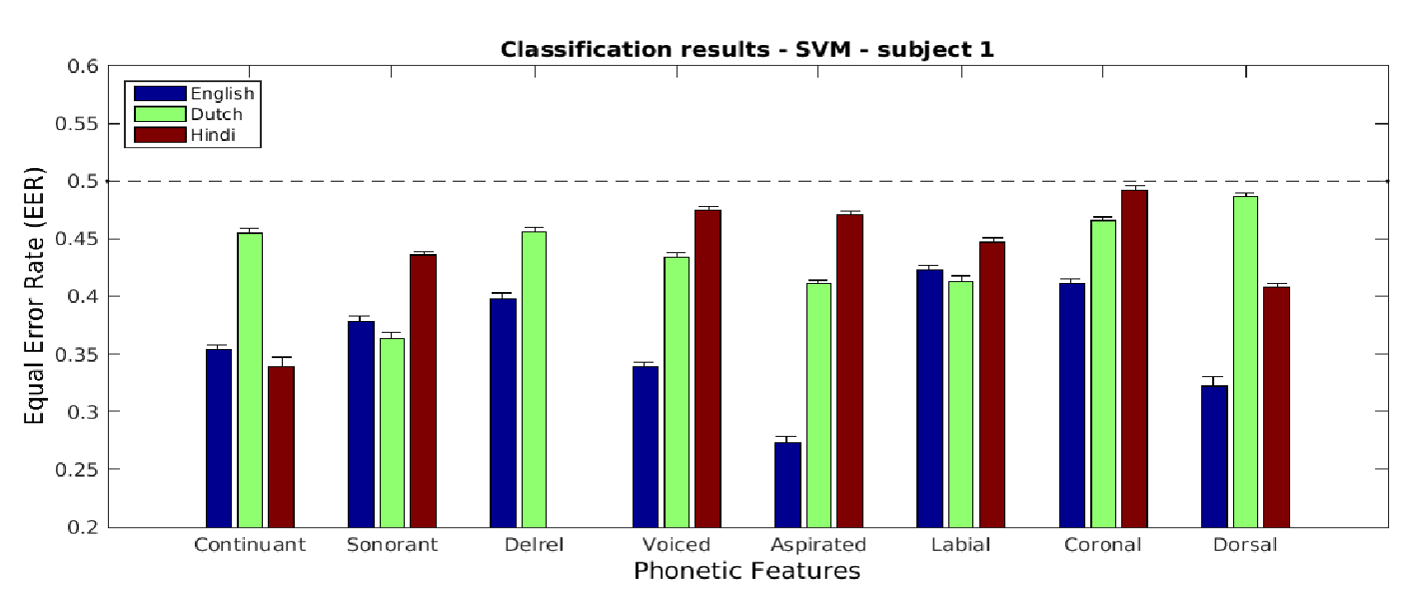
\includegraphics[width=5in]{../figs/diliberto_svmresults.png}}
  \caption{Classifiers were trained to observe EEG signals, and to
    classify the distinctive features of the phoneme being audited.
    Equal error rates are shown for English (the language used in
    training; train and test data did not overlap), Dutch, and Hindi
    (not used in training).}
  \label{fig:eeg_svm_eers}
\end{figure}

Eq.~\ref{eq:dfdist} defines a log-linear model of $\rho(\psi|\phi)$, the
probability that a non-English phoneme $\phi$ will be perceived as English
phoneme $\psi$.  Denote by $\rho_U(\psi|\phi)$ the model of
Eq.~\ref{eq:dfdist} with uniform weights for all distinctive features
($w_k=\alpha$, a tunable constant).  Denote by $\rho_{EEG}(\psi|\phi)$ the
same model, but with weights $w_k$ derived from EEG measurements
(Eq.~\ref{eq:eegdist}).  Fig.~\ref{fig:eeg_confusions} shows these
two confusion matrices: $\rho_U(\psi|\phi)$ on the left,
$\rho_{EEG}(\psi|\phi)$ on the right. The entropy of the
uniform weighting, $\rho_U(\psi|\phi)$, is too low: when a Dutch
phoneme $\phi$ has a nearest-neighbor $\psi^*(\phi)$ in English, then
few other phonemes are considered to be possible confusions.
$\rho_{EEG}(\psi|\phi)$ has a very different problem: since distinctive
feature classfiers have been trained for only a small set of
distinctive features,
there are large groups of phonemes whose confusion
probabilities can not be distinguished (giving the figure its
block-diagonal structure).  The faults of both models can be
ameliorated by interpolating them in some way, e.g., by computing the
linear interpolation
$\rho_I(\psi|\phi)=a\rho_U(\psi|\phi)+(1-a)\rho_{EEG}(\psi|\phi)$ for some
constant $0\le a\le 1$.

\begin{figure}
  \centerline{
    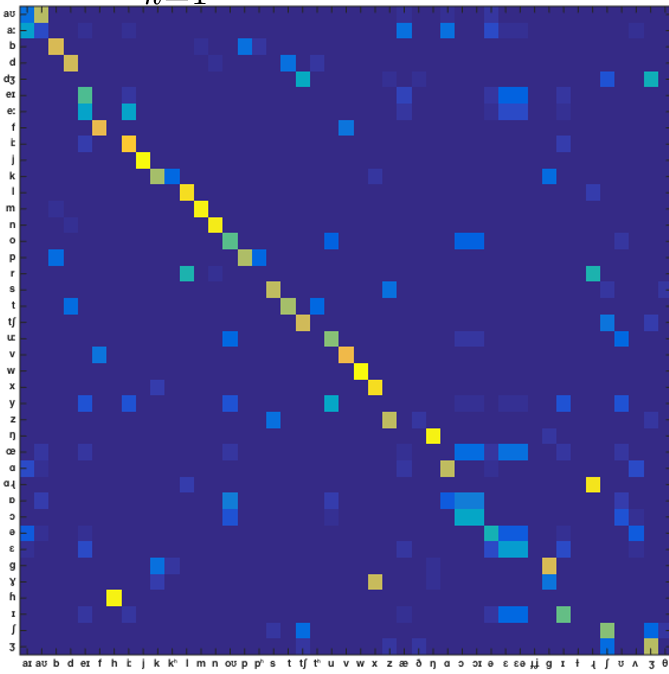
\includegraphics[width=3in]{../figs/mirbagheri_dist_features.png}
    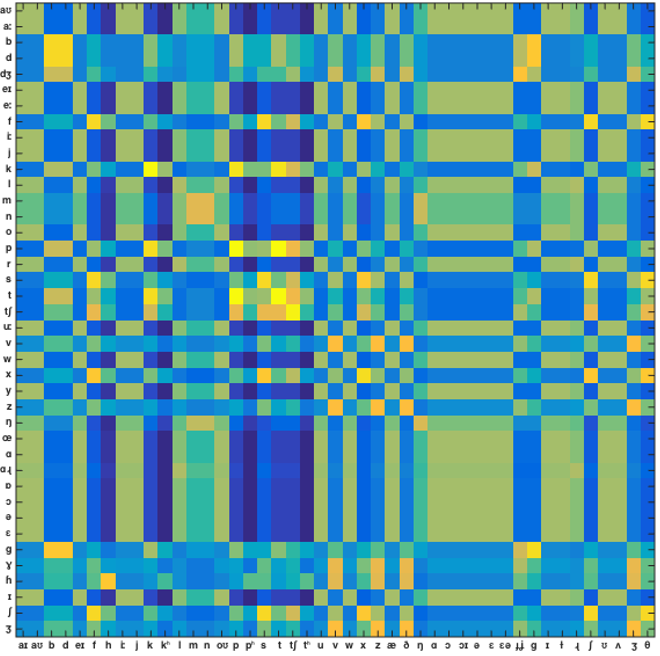
\includegraphics[width=3in]{../figs/mirbagheri_dist_eeg.png}
  }
  \caption{Phoneme confusion probabilities between English phonemes
    (column) and Dutch phonemes (row) using models in which the log
    probability is proportional to distance between the corresponding
    distinctive features.  Left: all features have the same
    weight.  Right: feature weights equal negative log error rate of
    EEG signal classifiers.}
  \label{fig:eeg_confusions}
\end{figure}
